\documentclass{article}
\usepackage{amsmath}
\usepackage{listings}
\usepackage{xcolor}
\usepackage{graphicx}
\usepackage{geometry}
\usepackage{hyperref}
\usepackage{tikz}
\usepackage{booktabs}
\usepackage{pgfplots}
\pgfplotsset{compat=1.18}
\usetikzlibrary{trees}
\geometry{margin=1in}

\title{Algorithm Analysis}
\author{}
\date{}

\definecolor{codegray}{rgb}{0.5,0.5,0.5}
\definecolor{backcolour}{rgb}{0.95,0.95,0.92}

\lstdefinestyle{cppstyle}{
  backgroundcolor=\color{backcolour},
  commentstyle=\color{codegray},
  keywordstyle=\color{blue},
  numberstyle=\tiny\color{codegray},
  stringstyle=\color{red},
  basicstyle=\ttfamily\footnotesize,
  breakatwhitespace=false,
  breaklines=true,
  captionpos=b,
  keepspaces=true,
  numbers=none,
  numbersep=5pt,
  showspaces=false,
  showstringspaces=false,
  showtabs=false,
  tabsize=2,
  language=C++
}

\begin{document}

\maketitle



\section{Why Analyze Algorithms?}

To compare how efficiently different algorithms solve the same problem, we analyze their use of time and space, primarily as a function of input size $n$.

\textbf{Motivating Example: Linear Search vs Binary Search}

Suppose you are given a sorted list of numbers and want to check whether a target number $x$ appears in the list.

\begin{itemize}
    \item \textbf{Linear Search:} Check each element one by one.
    \item \textbf{Binary Search:} Repeatedly divide the list in half and search the relevant half.
\end{itemize}

Both algorithms give the same result but can have vastly different performance. Analyzing them helps us compare their behavior without having to run code.
\section{Big-O Notation}

Big-O notation describes how the runtime of an algorithm grows in the worst case as the input size increases. It captures the dominant term and ignores constant factors.

\subsection{Example: Linear Search}
\begin{lstlisting}[style=cppstyle]
int linearSearch(const vector<int>& arr, int x) {
    for (int i = 0; i < arr.size(); i++) {
        if (arr[i] == x) return i;
    }
    return -1;
}
\end{lstlisting}

Worst-case: examine all $n$ elements.

\[
\Rightarrow \text{Time Complexity: } O(n)
\]

\subsection*{Example: Two Sum (Brute Force)}

Given an array and a target $k$, check if any two distinct elements sum to $k$.

\begin{lstlisting}[style=cppstyle]
bool twoSum(const vector<int>& arr, int k) {
    int n = arr.size();
    for (int i = 0; i < n; i++) {
        for (int j = i + 1; j < n; j++) {
            if (arr[i] + arr[j] == k) return true;
        }
    }
    return false;
}
\end{lstlisting}

Checks all pairs: $\approx \frac{n(n-1)}{2}$ comparisons.

\[
\Rightarrow \text{Time Complexity: } O(n^2)
\]

\subsection{Example: Matrix Multiplication}
\begin{lstlisting}[style=cppstyle]
void multiplyMatrices(const vector<vector<int>>& A,
                      const vector<vector<int>>& B,
                      vector<vector<int>>& C) {
    int n = A.size();
    for (int i = 0; i < n; i++) {
        for (int j = 0; j < n; j++) {
            C[i][j] = 0;
            for (int k = 0; k < n; k++) {
                C[i][j] += A[i][k] * B[k][j];
            }
        }
    }
}
\end{lstlisting}

\[
\Rightarrow \text{Time Complexity: } O(n^3)
\]

\section{The Master Method}

Divide-and-conquer algorithms often satisfy recurrences of the form:

\[
T(n) = a \cdot T\left(\frac{n}{b}\right) + f(n), \quad \text{where } f(n) = O(n^d),\ a \ge 1,\ b > 1
\]

Let $c = \log_b a$. Then:

\begin{itemize}
    \item \textbf{Case 1:} If $a > b^d$, then $T(n) = O(n^{\log_b a})$
    \item \textbf{Case 2:} If $a = b^d$, then $T(n) = O(n^d \log n)$
    \item \textbf{Case 3:} If $a < b^d$ and $f(n)$ dominates recursive cost, then $T(n) = O(n^d)$ (under regularity condition)
\end{itemize}

\subsection*{Example: Binary Search}
\begin{lstlisting}[style=cppstyle]
int binarySearch(const vector<int>& arr, int low, int high, int x) {
    if (low > high) return -1;
    int mid = (low + high) / 2;
    if (arr[mid] == x) return mid;
    else if (arr[mid] < x)
        return binarySearch(arr, mid + 1, high, x);
    else
        return binarySearch(arr, low, mid - 1, x);
}
\end{lstlisting}

Recurrence: $T(n) = T(n/2) + 1$

\begin{itemize}
    \item $a = 1,\ b = 2,\ f(n) = 1 = O(n^0) \Rightarrow d = 0$
    \item $\log_b a = \log_2 1 = 0 \Rightarrow$ Case 2
\end{itemize}

\[
\Rightarrow \text{Time Complexity: } O(\log n)
\]

\textbf{Recursion Tree Sketch:}
\[
T(n) \rightarrow T(n/2) \rightarrow T(n/4) \rightarrow T(n/8) \rightarrow \dots \rightarrow T(1)
\]



\begin{figure}[h!]
\centering
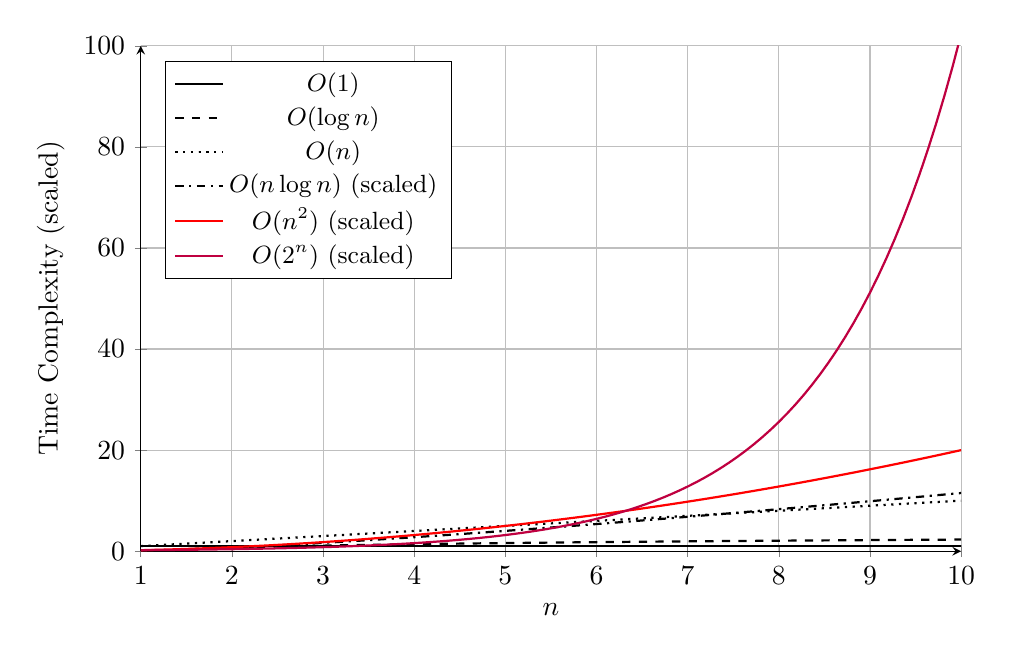
\begin{tikzpicture}
  \begin{axis}[
    width=12cm,
    height=8cm,
    xlabel={$n$},
    ylabel={Time Complexity (scaled)},
    legend pos=north west,
    ymin=0, ymax=100,
    xmin=1, xmax=10,
    domain=1:10,
    samples=100,
    grid=both,
    legend style={font=\small},
    axis lines=left
  ]

    \addplot[thick] {1};                         \addlegendentry{$O(1)$}
    \addplot[thick, dashed] {ln(x)};             \addlegendentry{$O(\log n)$}
    \addplot[thick, dotted] {x};                 \addlegendentry{$O(n)$}
    \addplot[thick, dashdotted] {x*ln(x)/2};     \addlegendentry{$O(n \log n)$ (scaled)}
    \addplot[thick, red] {x^2/5};                \addlegendentry{$O(n^2)$ (scaled)}
    \addplot[thick, purple] {2^x/10};            \addlegendentry{$O(2^n)$ (scaled)}

  \end{axis}
\end{tikzpicture}
\caption{Comparison of Common Growth Rates (scaled for visualization)}
\end{figure}

\subsection*{Execution Time at $n = 100$ (1 Operation = 1 Second)}

Assume that each basic operation takes 1 second. The table below shows the total runtime for different time complexities at $n = 100$:

\begin{center}
\begin{tabular}{|c|l|r|}
\hline
\textbf{Complexity} & \textbf{Expression at $n = 100$} & \textbf{Time (seconds)} \\
\hline
$O(1)$         & 1                         & 1 s \\
$O(\log n)$    & $\log_2(100) \approx 7$   & 7 s \\
$O(n)$         & 100                       & 100 s \\
$O(n \log n)$  & $100 \cdot 7 \approx 700$ & 700 s \\
$O(n^2)$       & $100^2 = 10,\!000$        & 2.8 hours \\
$O(2^n)$       & $2^{100} \approx 1.27 \times 10^{30}$ & $\sim 4 \times 10^{22}$ years \\
\hline
\end{tabular}
\end{center}

\textbf{Note:} 
\begin{itemize}
    \item $O(n^2)$ already becomes impractical beyond a few minutes.
    \item $O(2^n)$ is completely infeasible even for $n = 100$—illustrating the exponential explosion of brute-force algorithms.
\end{itemize}

\section{Other Asymptotic Notations}

\begin{tabular}{ll}
\toprule
Notation & Meaning \\
\midrule
$O(f(n))$  & Upper bound (at most proportional to $f(n)$) \\
$\Omega(f(n))$ & Lower bound (at least proportional to $f(n)$) \\
$\Theta(f(n))$ & Tight bound (exactly proportional to $f(n)$) \\
$o(f(n))$  & Strictly smaller (grows slower than $f(n)$) \\
$\omega(f(n))$ & Strictly larger (grows faster than $f(n)$) \\
\bottomrule
\end{tabular}

\section{Formal Proof Techniques}

\textbf{1. Definition of $O$-notation:}  
Show $T(n) \le c \cdot f(n)$ for all $n \ge n_0$, with some constant $c > 0$.

\textbf{Example:} If $T(n) \le 3n + 5$, we can choose $c = 4,\ n_0 = 5$ and prove:

\[
3n + 5 \le 4n \quad \text{for all } n \ge 5
\]

\textbf{2. Mathematical Induction:}  
Assume $T(k) \le c \cdot k$ for $k < n$, and show it holds for $n$.

\textbf{3. Substitution Method:}  
Assume a bound (e.g., $T(n) \le c \cdot n$), substitute into the recurrence, and verify it holds.

\textbf{4. Recursion Tree Method:}  
Unroll the recurrence into a tree, compute work per level, and sum total work.

\textbf{5. Proving Tight Bounds ($\Theta$):}  
Show both upper and lower bounds exist:

\[
c_1 \cdot f(n) \le T(n) \le c_2 \cdot f(n), \quad \text{for all } n \ge n_0
\]

\end{document}